\chapter{Perancangan}

\section{Rancangan Alur Program}
Secara garis besar program terbagi menjadi dua proses yang saling terhubung. Proses pertama merupakan proses \textit{clustering} untuk membuat model. Proses \textit{clustering} menerima \textit{dataset} dalam bentuk \textit{file} gambar, melakukan ekstraksi fitur lokal dari gambar-gambar tersebut dan membuat model. Proses yang kedua adalah proses OIR yang dilakukan dengan menggunakan metode BSIS. Proses kedua ini menerima \textit{file} model yang dihasilkan oleh proses \textit{clustering} dan menggunakan model tersebut untuk dapat melakukan pengenalan terhadap gambar masukan. Rancangan alur program ini dapat dilihat pada diagram di Gambar~\ref{fig:rancangan_alur_program}.
\begin{figure}[H]
	\centering
	\includegraphics[width=\textwidth]{rancangan\_alur\_program.png}
	\caption{Rancangan alur program pada penelitian ini.}
	\label{fig:rancangan_alur_program}
\end{figure}
Berdasarkan dari diagram pada Gambar~\ref{fig:rancangan_alur_program} tersebut program akan terbagi menjadi 2 modul. Modul pertama merupakan modul \textit{clustering} yang implementasinya dijelaskan pada \ref{sec:rancangan_clustering}. Modul yang kedua adalah modul BSIS yang implementasinya dijelaskan pada \ref{sec:rancangan_bsis}. Selain itu untuk model yang dihasilkan oleh proses \textit{clustering} dan digunakan untuk proses BSIS akan dijelaskan pada \ref{sec:clustermodel_class}.

\section{Rancangan Implementasi Metode Clustering Pembuatan Model} 
\label{sec:rancangan_clustering}
Metode \textit{clustering} diimplementasi dalam sebuah modul Python yang menerima \textit{file} dalam bentuk gambar dan menghasilkan sebuah \textit{dataframe} yang berisi detail-detail fitur lokal dari gambar. Gambar-gambar masukan yang digunakan perlu untuk memiliki sebuah struktur \textit{folder} tertentu. Keterangan struktur \textit{folder} masukan serta fungsi-fungsi dalam modul hingga struktur \textit{file} keluaran akan dijelaskan pada subbab-subbab berikut ini.

\subsection{Rancangan Struktur Folder}
\label{subsec:struktur_folder_clustering}
Rancangan struktur \textit{folder} yang diperlukan untuk dapat digunakan sebagai masukan pada modul \textit{clustering} adalah sebagai berikut, dapat dilihat pada Gambar~\ref{fig:struktur_folder}.
\begin{figure}[H]
	\centering
	\includegraphics[scale=0.6]{struktur\_folder.png}
	\caption{Rancangan struktur \textit{folder} untuk pembuatan model.}
	\label{fig:struktur_folder}
\end{figure}
Gambar tersebut menunjukkan struktur \textit{folder} masukan yang diperlukan pada modul ini. \textit{Folder} yang paling atas merupakan \textit{folder} utama yang juga menjadi nama \textit{dataset}. \textit{Folder} utama akan berisi beberapa \textit{subfolder} yang menunjukkan kelas dari gambar. Setiap \textit{subfolder} ini berisi beberapa \textit{file} gambar yang merupakan bagian dari kelas tersebut. Gambar-gambar \textit{dataset} yang sudah dalam struktur seperti ini dapat digunakan dalam proses \textit{clustering}

\subsection{Rancangan Proses Clustering}
\label{subsec:rancangan_proses_clustering}
Proses \textit{clustering} menerima \textit{dataset} gambar sesuai dengan struktur \textit{folder} yang telah dijelaskan sebelumnya pada \ref{subsec:struktur_folder_clustering}. Dari \textit{dataset} tersebut diproses dan dihasilkan \textit{dataframe} yang berisi deskriptor dari setiap fitur lokal serta nilai keunikan dan konsistensi. Langkah-langkah yang dilakukan proses ini serta hasil keluaran dari setiap langkah dapat dilihat pada diagram di Gambar~\ref{fig:dfd_clustering}.
\begin{figure}[H]
	\centering
	\includegraphics[width=\textwidth]{dfd\_clustering.png}
	\caption{Tahapan proses \textit{clustering} hingga didapat nilai keunikan dan konsistensi.}
	\label{fig:dfd_clustering}
\end{figure}
Proses dalam Modul Clustering ini dapat dilakukan dengan menggunakan dua tipe metode ekstraksi fitur lokal yaitu SIFT dan ORB. SIFT dan ORB memiliki bentuk dan isi deskriptor fitur lokal yang berbeda, di mana deskriptor SIFT merupakan vektor bilangan bulat sedangkan deskriptor ORB adalah vektor bilangan biner. Perbedaan bentuk dan isi vektor deskriptor tersebut menyebabkan perlunya dibuat implementasi yang berbeda untuk SIFT dan ORB. Beberapa perbedaan implementasi untuk SIFT dan ORB adalah sebagai berikut:
\begin{itemize}
	\item Di langkah 2 dan 3 \textit{clustering} untuk SIFT dilakukan dengan menggunakan metrik jarak Euclidean, sedangkan untuk ORB metrik jarak yang digunakan adalah Hamming.
	\item Di langkah 2 saat menggunakan SIFT dihitung \textit{centroid} untuk setiap hasil \textit{clustering} tiap gambar, sedangkan pada ORB yang dihitung adalah \textit{medoid}.
\end{itemize}
Selain dari perbedaan-perbedaan tersebut langkah implementasi yang dilakukan sama, baik untuk metode ekstraksi fitur lokal SIFT maupun ORB. Proses penghitungan nilai keunikan dapat dilihat pada Pseudocode~\ref{alg:uniqueness}. \\

\begin{algorithm}[H]
	\caption{UNIQUENESS}
	\label{alg:uniqueness}
	\KwIn{\begin{itemize}[nosep]
			\item \textit{D}: \textit{dataframe} yang memiliki kolom berisi nama gambar (\texttt{img}), kelompok gambar (\texttt{img\_class}), dan label \textit{cluster} (\texttt{cluster\_label}).
	\end{itemize}}
	\KwOut{list berisi nilai keunikan}
	\begin{algorithmic}[1]
		\STATE buat \textit{dictionary} \textit{class\_count}
		\STATE kelompokan \textit{D} berdasarkan kolom \texttt{cluster\_label}.
		\FOR{semua \texttt{cluster\_label} \textit{\textbf{c}} kelompok \texttt{cluster\_label}}
		\STATE buat variabel \textit{\textbf{o}} yang berisi semua elemen \textit{D} yang memiliki \texttt{cluster\_label} \textit{\textbf{c}}
		\STATE hapus baris dalam \textit{\textbf{o}} yang nilai kolom \texttt{img}-nya duplikat sehingga untuk setiap nilai \texttt{img} yang berbeda hanya muncul satu kali.
		\STATE hitung jumlah setiap \texttt{img\_class} yang ada dalam \textit{\texttt{o}} dan bagi nilainya dengan jumlah elemen dalam \textit{\textbf{o}}
		\STATE masukkan nilai penghitungan jumlah tiap \texttt{img\_class} ke dalam sebuah \textit{dictionary} dua tingkat dengan \textit{key} pertama adalah \textit{\textbf{c}} dan \textit{key} kedua adalah isi \texttt{img\_class}.
		\ENDFOR
		\STATE buat \textit{list} \textit{\textbf{uniqueness}}
		\FOR{baris \textit{\texttt{r}} dalam \textit{D}}
		\STATE ambil nilai keunikan dari \textit{\textbf{class\_count}} dengan menggunakan \texttt{cluster\_label} dan \texttt{img\_class} sebagai \textit{key}
		\STATE masukkan nilai keunikan tersebut ke \textit{\textbf{uniqueness}}. 
		\ENDFOR
		\RETURN \textit{\textbf{uniqueness}}
	\end{algorithmic}
\end{algorithm}
Sedangkan untuk penghitungan nilai konsistensi mengikuti proses pada Pseudocode~\ref{alg:consistency}. \\
\begin{algorithm}[H]
	\caption{CONSISTENCY}
	\label{alg:consistency}
	\KwIn{\begin{itemize}[nosep]
			\item \textit{D}: \textit{dataframe} yang memiliki kolom berisi nama gambar (\texttt{img}), kelompok gambar (\texttt{img\_class}), dan label \textit{cluster} (\texttt{cluster\_label}).
	\end{itemize}}
	\KwOut{\textit{list} berisi nilai konsistensi}
	\begin{algorithmic}[1]
		\STATE kelompokan \textit{D} berdasarkan \texttt{cluster\_label} dan \texttt{img\_class}.
		\STATE hitung jumlah gambar yang unik untuk tiap kelompok. Masukkan hasilnya ke dalam \textit{dictionary} dua tingkat \textit{\textbf{d}} yang memiliki \textit{key} pertama adalah isi dari \texttt{cluster\_label} dan \textit{key} keduanya adalah isi dari \texttt{img\_class}.
		\STATE buat \textit{list} \textit{\textbf{consistency}}
		\FOR{baris \textit{\textbf{r}} dalam \textit{D}}
		\STATE buat variabel \textit{\textbf{v}} dengan mengambil nilai \textit{\texttt{d}} menggunakan \texttt{cluster\_label} dan \texttt{img\_class} dari \textit{\textbf{r}} sebagai \textit{key}.
		\STATE bagi nilai \textit{\textbf{v}} dengan jumlah gambar pada \textit{dataset} yang kelasnya sama dengan \texttt{img\_class} dari \textit{\textbf{r}}.
		\STATE masukan \textit{\textbf{v}} ke \textit{\textbf{consistency}}
		\ENDFOR
		\RETURN \textit{\textbf{consistency}}
	\end{algorithmic}
\end{algorithm}
Proses yang dilakukan pada Gambar~\ref{fig:dfd_clustering} akan menghasilkan sebuah \textit{dataframe} dengan ketentuan kolom seperti pada Tabel~\ref{tab:df_clustering}. \textit{Dataframe} tersebut disimpan ke dalam \textit{file} \texttt{pickle} dengan menggunakan \textit{library} Pickle di Python.
\begin{table}[H]
	\begin{tabular}{|p{0.25\textwidth}|p{0.25\textwidth}|p{0.45\textwidth}|}
		\hline
		Nama Kolom      & Kelompok Kolom                            & Deskripsi                                                                                                   \\ \hline
		0               & \multirow{5}{0.45\textwidth}{Deskriptor}               & \multirow{5}{0.45\textwidth}{Berjumlah 128 kolom yang masing-masing merupakan satu elemen dalam vektor deskriptor SIFT.} \\ \cline{1-1}
		1               &                                           &                                                                                                             \\ \cline{1-1}
		...             &                                           &                                                                                                             \\ \cline{1-1}
		126             &                                           &                                                                                                             \\ \cline{1-1}
		127             &                                           &                                                                                                             \\ \hline
		img             & \multirow{2}{*}{Informasi Gambar}         & Nama gambar asal fitur lokal                                                                                \\ \cline{1-1} \cline{3-3} 
		img\_class      &                                           & Kelas dari gambar asal fitur lokal                                                                          \\ \hline
		cluster\_label  & \multirow{2}{*}{Label \textit{Cluster}}            & Label \texttt{cluster} dari hasil \textit{clustering} per gambar                                                              \\ \cline{1-1} \cline{3-3} 
		cluster2\_label &                                           & Label \textit{cluster} dari hasil \texttt{clustering} \textit{centroid}                                                                \\ \hline
		uniqueness      & \multirow{2}{*}{Nilai Hasil Penghitungan} & Nilai keunikan fitur lokal yang didapat dari hasil \textit{clustering}                                               \\ \cline{1-1} \cline{3-3} 
		consistency     &                                           & Nilai konsistensi fitur lokal yang didapat dari hasil \textit{clustering}                                            \\ \hline
		point\_x    & \multirow{7}{*}{Atribut \textit{keypoint}}         & Koordinat x dari \textit{keypoint}                                                                                   \\ \cline{1-1} \cline{3-3} 
		point\_y    &                                           & Koordinat y dari \textit{keypoint}                                                                                   \\ \cline{1-1} \cline{3-3} 
		size            &                                           & Diameter daerah di sekitar \textit{keypoint} yang diperiksa                                                          \\ \cline{1-1} \cline{3-3} 
		angle           &                                           & Orientasi dari \textit{keypoint}                                                                                     \\ \cline{1-1} \cline{3-3} 
		response        &                                           & Tingkat respon yang menyatakan seberapa kuat \textit{keypoint}                                                       \\ \cline{1-1} \cline{3-3} 
		octave          &                                           & Oktaf di mana \textit{keypoint} tersebut didapat                                                                     \\ \cline{1-1} \cline{3-3} 
		class\_id       &                                           & Kelas objek yang menyatakan kelompok dari \textit{keypoint} jika dikelompokkan                                       \\ \hline
	\end{tabular}
	\caption{Rincian kolom dari \textit{dataframe} yang dihasilkan modul proses \textit{clustering}.}
	\label{tab:df_clustering}
\end{table}
Rancangan proses \textit{clustering} ini dibuat ke dalam dua buah \textit{script} Python dengan nama \texttt{clustering\_sift.py} dan \texttt{clustering\_orb.py}. Kedua \textit{script} tersebut berguna untuk melakukan proses \textit{clustering} sesuai dengan metode ekstraksi fitur lokalnya SIFT atau ORB. Baik \texttt{clustering\_sift.py} dan \texttt{clustering\_orb.py} dapat dijalankan dengan menerima dua argumen berikut:
\begin{itemize}
	\item \texttt{dir}: lokasi tempat \textit{dataset} gambar yang akan dibuat modelnya. Direktori harus memiliki struktur \textit{folder} yang sesuai dengan \ref{subsec:struktur_folder_clustering}.
	\item \texttt{maxsize}: ukuran sisi maksimum dari gambar \textit{dataset}. Gambar akan diperkecil jika ukuran panjang atau lebarnya melebihi nilai ini.
\end{itemize}
Contoh \textit{command} untuk menjalankan \textit{script} proses \textit{clustering} adalah sebagai berikut:
\begin{lstlisting}[language=bash, 
	basicstyle=\normalsize,
	frame=none,
	numbers=none]
	python clustering_sift.py --dir datasets/gsv --maxsize 600
\end{lstlisting}

\textit{Script} tersebut akan menghasilkan sebuah \textit{file} yang dapat dibaca oleh kelas \texttt{ClusterModel}. Kelas \texttt{ClusterModel} sendiri akan dijelaskan pada subbab berikut ini.
 
\section{Rancangan Kelas ClusterModel}
\label{sec:clustermodel_class}
Kelas \texttt{ClusterModel} adalah kelas yang berguna untuk menyimpan dan memproses model yang dihasilkan oleh proses \textit{clustering} untuk digunakan pada BSIS. Kelas ini menyimpan data-data fitur lokal serta \textit{keypoint} dan nilai-nilai yang didapat dari hasil \textit{clustering}. Kelas memiliki \textit{method} untuk menyimpan model kedalam sebuah \textit{file} dan juga \textit{method} untuk membaca model dari \textit{file}. 

Kelas ini juga berguna sebagai perantara antara proses \textit{clustering} dan BSIS. Kelas memilik i\textit{method} untuk menghasilkan fitur-fitur lokal yang sudah disaring berdasarkan nilai konsistensi dan keunikan. Fitur-fitur lokal yang dihasilkan ini dalam format yang dapat dibaca oleh kelas BSIS. Diagram kelas \texttt{ClusterModel} beserta \textit{inner-class}-nya dapat dilihat pada Gambar~\ref{fig:clustermodel_class}.
\begin{figure}[H]
	\centering
	\includegraphics[width=\textwidth]{clustermodel\_class.png}
	\caption{Diagram kelas \texttt{ClusterModel}.}
	\label{fig:clustermodel_class}
\end{figure}
Kelas ini terdiri dari kelas \texttt{ClusterModel} dan tiga \textit{inner-class} yang masing-masing memiliki fungsi sebagai berikut:
\begin{itemize}
	\item \texttt{Meta}: menyimpan informasi dasar tentang model yang dihasilkan. Informasi yang disimpan meliputi jumlah data, ukuran maksimum gambar, tipe deskriptor, nama-nama kelas gambar, dan jumlah gambar tiap kelas. 
	\item \texttt{Descriptor}: merupakan enumerasi yang menyimpan dua tipe deskriptor yang dapat digunakan. Tipe deskriptor ini akan berpengaruh pada format data masukan saat membuat objek \texttt{ClusterModel}.
	\item \texttt{LocalFeature}: menyimpan keluaran fungsi \texttt{get\_local\_features} dari  \texttt{ClusterModel} dengan format tertentu. Format ini merupakan format yang digunakan sebagai data masukan pada kelas BSIS.
\end{itemize}
Kelas \texttt{ClusterModel} sendiri memiliki beberapa fungsi penting sebagai berikut:
\begin{itemize}
	\item \texttt{from\_dataframe}: fungsi yang digunakan untuk membuat objek \texttt{ClusterModel} dari \textit{dataframe} yang berisi kolom-kolom seperti pada Tabel~\ref{tab:df_clustering}.
	\item \texttt{get\_local\_features}: fungsi untuk mengembalikan sebuah \textit{list} berisi objek \texttt{LocalFeature}. Fungsi ini digunakan untuk menghasilkan masukkan yang dapat digunakan oleh kelas BSIS.
	\item \texttt{get\_dataframe}: fungsi untuk mengembalikan data yang disimpan dalam objek \textit{ClusterModel} dalam bentuk \textit{dataframe}. Fungsi ini berguna untuk melakukan analisis pada hasil proses \textit{clustering} yang telah tersimpan sebagai objek \texttt{ClusterModel}.
\end{itemize}


%Kelas \texttt{ClusterModel} adalah kelas yang digunakan untuk membaca file \texttt{pickle} berisi \textit{dataframe} yang dihasilkan dari proses pada \ref{subsec:rancangan_proses_clustering}. Kelas ini membaca data dan memiliki beberapa \textit{method} yang digunakan untuk mengubah data dalam \textit{dataframe} menjadi format yang dapat digunakan. Diagram untuk kelas \texttt{ClusterModel} dapat dilihat pada Gambar~\ref{fig:clustermodel_class}

%Atribut \texttt{data} pada kelas tersebut adalah \textit{dataframe} yang dihasilkan dari modul sebelumnya dan dibaca dengan kelas ini. Kegunaan fungsi-fungsi dari kelas \texttt{ClusterModel} adalah sebagai berikut:
%\begin{enumerate}
%	\item \texttt{\_\_init\_\_} \\
%	Fungsi konstruktor kelas \texttt{ClusterModel} menerima parameter \texttt{path} yang merupakan direktori tempat \textit{file} \textit{dataframe} yang ingin digunakan. Fungsi akan memasukkan \textit{file} pada direktori \texttt{path} ke atribut \texttt{data}.
%	\item \texttt{get\_keypoints\_with\_mapper} \\
%	Fungsi menyaring \texttt{data} dengan menetapkan batas bawah pada kolom \texttt{uniqueness} dan \texttt{consistency}. Fungsi ini memberikan tiga keluaran, yaitu sebuah \textit{list} berisi objek \textit{keypoint}, sebuah \textit{array} 2 dimensi berisi deskriptor, dan sebuah \textit{dictionary} yang menunjukkan gambar asal dari setiap \textit{keypoint}.
%	\item \texttt{get\_keypoint} \\
%	Fungsi berguna untuk membuat objek \textit{keypoint} dari sebuah baris \textit{dataframe}. Fungsi ini mengambil nilai dari kolom \texttt{kp\_point\_x}, \texttt{kp\_point\_y}, \texttt{size}, \texttt{angle}, \texttt{response}, \texttt{octave}, \texttt{class\_id} dan membuat objek \textit{keypoint} dari nilai-nilai tersebut.
%	\item \texttt{get\_descriptor} \\
%	Fungsi mengambil 128 kolom pertama dari sebuah baris \textit{dataframe} dan mengembalikan \textit{list} berisi nilai-nilai tersebut.
%\end{enumerate}

\section{Rancangan Kelas Util}
Kelas \textit{Util} berisi fungsi-fungsi pembantu yang digunakan pada kelas-kelas lainnya. Fungsi-fungsi ini berguna untuk mempermudah proses komputasi saat menggunakan kelas lainnya dan saat melakukan analisis. Fungsi-fungsi dalam kelas \textit{Util} dapat dilihat pada diagram di Gambar~\ref{fig:util_class}.
\begin{figure}[H]
	\centering
	\includegraphics[width=\textwidth]{util\_class.png}
	\caption{Diagram kelas \texttt{Util}}
	\label{fig:util_class}
\end{figure}
Beberapa fungsi penting dari kelas \texttt{Util} adalah sebagai berikut:
\begin{enumerate}
	\item \texttt{get\_image} \\
	Fungsi untuk memuat gambar dari \textit{file}. Parameter \texttt{bw} menyatakan apakah gambar yang dimuat akan diubah menjadi format \textit{grayscale}. Sedangkan untuk \texttt{maxwidth} dan \texttt{maxheight} digunakan untuk mengatur ukuran dari gambar.
	\item \texttt{get\_all\_image} \\
	Fungsi untuk memuat semua gambar dalam suatu \textit{folder}. Fungsi ini memanggil fungsi \texttt{get\_image} untuk semua \textit{file} gambar dalam \textit{folder} di \texttt{directory}.
	\item \texttt{get\_dataset} \\
	Fungsi untuk memuat semua \textit{file} gambar dengan fungsi \texttt{get\_image} dari \textit{file} yang tersusun sesuai struktur \textit{folder} seperti yang dijelaskan pada \ref{subsec:struktur_folder_clustering}. Fungsi ini digunakan untuk mendapatkan gambar masukkan pada \ref{subsec:rancangan_proses_clustering}.
	\item \texttt{agglo\_cluster} \\
	Fungsi untuk melakukan \textit{Agglomerative Clustering} pada \textit{dataset}. Fungsi akan mengembalikan sebuah \textit{array} yang berisi label \textit{cluster}. Fungsi ini digunakan untuk melakukan \textit{clustering} per gambar dan \textit{clustering} \textit{centroid} pada analisis yang dilakukan di \ref{sec:analisis_sifat} dengan mengikuti rancangan pada \ref{subsec:rancangan_proses_clustering}.
	\item \texttt{show\_keypoints} \\
	Fungsi untuk menampilkan \textit{keypoint} pada gambar. Fungsi digunakan untuk melakukan visualisasi \textit{keypoint} di gambar yang dilakukan pada \ref{sec:analisis_sifat}.
	\item \texttt{show\_matches} \\
	Fungsi untuk menampilkan pasangan \textit{keypoint} dari dua gambar. Fungsi ini digunakan untuk menampilkan pasangan \textit{keypoint} yang kuat pada analisis di \ref{sec:analisis_poi}.
\end{enumerate}


\section{Rancangan Kelas-kelas Implementasi BSIS}
\label{sec:rancangan_bsis}
Implementasi BSIS dibuat dalam sebuah \textit{package} yang didalamnya berisi beberapa kelas yang saling berhubungan. Kelas-kelas beserta fungsi dalam kelas yang ada di \textit{package} BSIS dapat dilihat pada Gambar~\ref{fig:bsis_package}. Kelas-kelas pada \textit{package} ini digunakan untuk melakukan BSIS pada \ref{sec:analisis_bsis} dengan memanggil kelas \texttt{BSIS}.
\begin{figure}[H]
	\centering
	\includegraphics[width=\textwidth]{bsis\_package.png}
	\caption{Diagram \textit{Package} \texttt{bsis}.}
	\label{fig:bsis_package}
\end{figure}
Untuk melakukan BSIS terhadap sebuah gambar pertama perlu dibuat sebuah objek kelas \texttt{BSIS}. Pembuatan objek BSIS menerima satu masukan yaitu sebuah \textit{dictionary} yang berisi \textit{list} \textit{keypoint} dan \textit{array} deskriptor. Setelah itu isi \texttt{train\_set} dengan memanggil fungsi \texttt{set\_train\_data}. Fungsi \texttt{set\_train\_data} menerima \textit{list} yang dihasilkan oleh fungsi \texttt{get\_local\_features} dari kelas \texttt{ClusterModel}. Setelah objek BSIS telah mendapatkan gambar masukan dan \textit{dataset} \textit{train} panggil fungsi \texttt{run} untuk menjalankan proses identifikasi. Setelah proses identifikasi selesai objek BSIS tersebut akan menyimpan hasil dari identifikasi.

Fungsi-fungsi lain dalam \textit{package} tersebut dipanggil oleh kelas \texttt{BSIS} saat pemrosesan, kegunaan masing-masing kelas adalah sebagai berikut:
\begin{enumerate}
	\item \texttt{TrainSet} \\
	Kelas untuk mengatur \textit{dataset} yang digunakan pada kelas \texttt{BSIS}.
	\item \texttt{Pair} \\
	Kelas untuk menyimpan pasangan fitur lokal. Fungsi \texttt{make\_pairs\_kdtree} dari \texttt{BSIS} mengembalikan sebuah \textit{list} yang berisi objek \texttt{Pair}.
	\item \texttt{BPair} \\
	\makebox[\linewidth][s]{Kelas untuk menyimpan sebuah \textit{sequence} \texttt{Pair}. Digunakan pada tahap verifikasi} \newline (\texttt{find\_best\_subsequence}) di \texttt{BSIS\_Verify}. \textit{Sequence} \texttt{Pair} diimplementasikan dalam bentuk objek \texttt{BPair} dalam objek \texttt{BPair}. Atribut \texttt{prev} dalam \texttt{BPair} akan diisi dengan objek \texttt{BPair} lain yang juga dapat memiliki objek \texttt{BPair} di atribut \texttt{prev}-nya. 
	\item \texttt{BSIS\_Verify} \\
	Kelas untuk melakukan verifikasi geometris dari pasangan fitur lokal yang dihasilkan oleh fungsi \texttt{make\_pairs\_kdtree} dari BSIS. Pada kelas ini pertama dilakukan pembuatan \textit{list} 2 dimensi yang mengurutkan pasangan berdasarkan \textit{order} x (urutan kemunculan \textit{keypoint} di sumbu x) dari \textit{keypoint} di gambar \textit{train} yang dilakukan oleh fungsi \texttt{get\_pair\_list\_ordered}. \textit{List} yang dihasilkan oleh fungsi \texttt{get\_pair\_list\_ordered} memiliki elemen yang merupakan \textit{list} juga dengan panjang yang dapat berbeda-beda dan isinya merupakan objek \texttt{BPair} yang menyimpan informasi \textit{Pair} dan atribut \texttt{prev}-nya kosong (berisi \texttt{None}). Setelah itu dilakukan verifikasi pada \textit{list} tersebut dengan menggunakan fungsi \texttt{find\_best\_subsequence}. Proses verifikasi pada \texttt{find\_best\_subsequence} didefinisikan pada Pseudocode~\ref{alg:find_best_subsequence}. \\
\end{enumerate}
\begin{algorithm}[H]
	\caption{FIND\_BEST\_SUBSEQUENCE}
	\label{alg:find_best_subsequence}
	\KwIn{\begin{itemize}[nosep]
			\item \textit{D}: sebuah \textit{list} dengan setiap elemennya merupakan \textit{list} berisi objek \texttt{BPair}, dapat memiliki panjang yang berbeda-beda.
	\end{itemize}}
	\KwOut{\textit{sequence} \texttt{BPair} yang merupakan pasangan yang konsisten secara geometris dan nilai total bobotnya paling tinggi}
	\begin{algorithmic}[1]
		\STATE buat objek \texttt{BPair} \textit{\textbf{best\_subsequence}}.
		\STATE buat \textit{dictionary} \textit{\textbf{best\_per\_order}}.
		\FOR{\textit{\textbf{i}}=1 hingga LENGTH(\textit{D})}
			\FOR{\textit{\textbf{j}}=1 hingga LENGTH(\text{D[\textit{\textbf{i}}]})}
				\IF{ORDER(\textit{D}[\textit{\textbf{i}}][\textit{\textbf{j}}]) tidak ada di \textit{\textbf{best\_per\_order}}}
					\STATE isi \textit{\textbf{best\_per\_order}}[ORDER(\textit{D}[\textit{\textbf{i}}][\textit{\textbf{j}}])] dengan \textit{D[\textit{\textbf{i}}][\textit{\textbf{j}}]}
				\ELSIF{BTS(\textit{D}[\textit{\textbf{i}}][\textit{\textbf{j}}]) lebih besar dari BTS(\textit{\textbf{best\_per\_order}}[ORDER(\textit{D}[\textit{\textbf{i}}][\textit{\textbf{j}}])])}
					\STATE isi \textit{\textbf{best\_per\_order}}[ORDER(\textit{D}[\textit{\textbf{i}}][\textit{\textbf{j}}])] dengan \textit{D[\textit{\textbf{i}}][\textit{\textbf{j}}]}
				\ENDIF
				\STATE objek \texttt{BPair} \textit{\textbf{dBestPrev}}
				\FOR{\textit{\textbf{ord}}=1 hingga ORDER(\textit{D}[\textit{\textbf{i}}][\textit{\textbf{j}}])}
					\IF{\textit{\textbf{ord}} ada di \textit{\textbf{best\_per\_order}}}
						\IF{BTS(\textit{\textbf{best\_per\_order}}) lebih besar dari BTS(\textit{\textbf{dBestPrev}})}
							\STATE isi \textit{\textbf{dBestPrev}} dengan \textit{\textbf{best\_per\_order}}[\textit{\textbf{ord}}]
						\ENDIF
					\ENDIF
				\ENDFOR
				\STATE isi BTS(\textit{D[\textit{\textbf{i}}][\textit{\textbf{j}}]}) dengan WEIGHT(\textit{D}[\textit{\textbf{i}}][\textit{\textbf{j}}]) + BTS(\textit{\textbf{dBestPrev}})
				\STATE isi PREV(\textit{D[\textit{\textbf{i}}][\textit{\textbf{j}}]}) dengan \textit{\textbf{dBestPrev}}
				\IF{BTS(\textit{D[\textit{\textbf{i}}][\textit{\textbf{j}}]}) + WEIGHT(\textit{D[\textit{\textbf{i}}][\textit{\textbf{j}}]}) > BTS(\textit{\textbf{best\_subsequence}}) + WEIGHT(\textit{\textbf{best\_subsequence}})}
					\STATE isi \textit{\textbf{best\_subsequence}} dengan \textit{D[\textit{\textbf{i}}][\textit{\textbf{j}}]}
				\ENDIF
			\ENDFOR
		\ENDFOR
		\RETURN \textit{\textbf{best\_subsequence}}
	\end{algorithmic}
\end{algorithm}

\section{Rancangan Perangkat Lunak BSIS}
Untuk lebih mudah melakukan BSIS pada sebuah gambar masukkan, dibuat sebuah perangkat lunak dengan GUI yang dapat melakukan identifikasi gambar masukkan dengan BSIS. Perangkat lunak yang dibuat memiliki fitur sebagai berikut:
\begin{itemize}
	\item Memilih model yang ingin digunakan untuk identifikasi gambar masukkan.
	\item Memilih gambar masukkan yang ingin diidentifikasi.
	\item Menentukan nilai \textit{threshold} untuk konsistensi dan keunikan.
	\item Melakukan identifikasi pada gambar yang telah dipilih, dengan menggunakan model serta \textit{threshold} yang telah ditentukan.
\end{itemize}
Saat dilakukan identifikasi pada gambar, perangkat lunak akan melakukan BSIS pada gambar masukkan dengan menggunakan \textit{dataset} berdasarkan model dan nilai \textit{threshold} yang telah dipilih. Perangkat lunak lalu akan menampilkan hasil beberapa pasangan yang didapat diurutkan berdasarkan total bobotnya. Hasil yang dikembalikan berupa nama gambar, total bobot, dan gambar yang menunjukkan pasangan \textit{keypoint}-nya. Untuk memenuhi fungsionalitas tersebut dibikin perangkat lunak dengan rancangan tampilan seperti yang dapat dilihat pada Gambar~\ref{fig:rancangan_ui}
\begin{figure}[H]
	\centering
	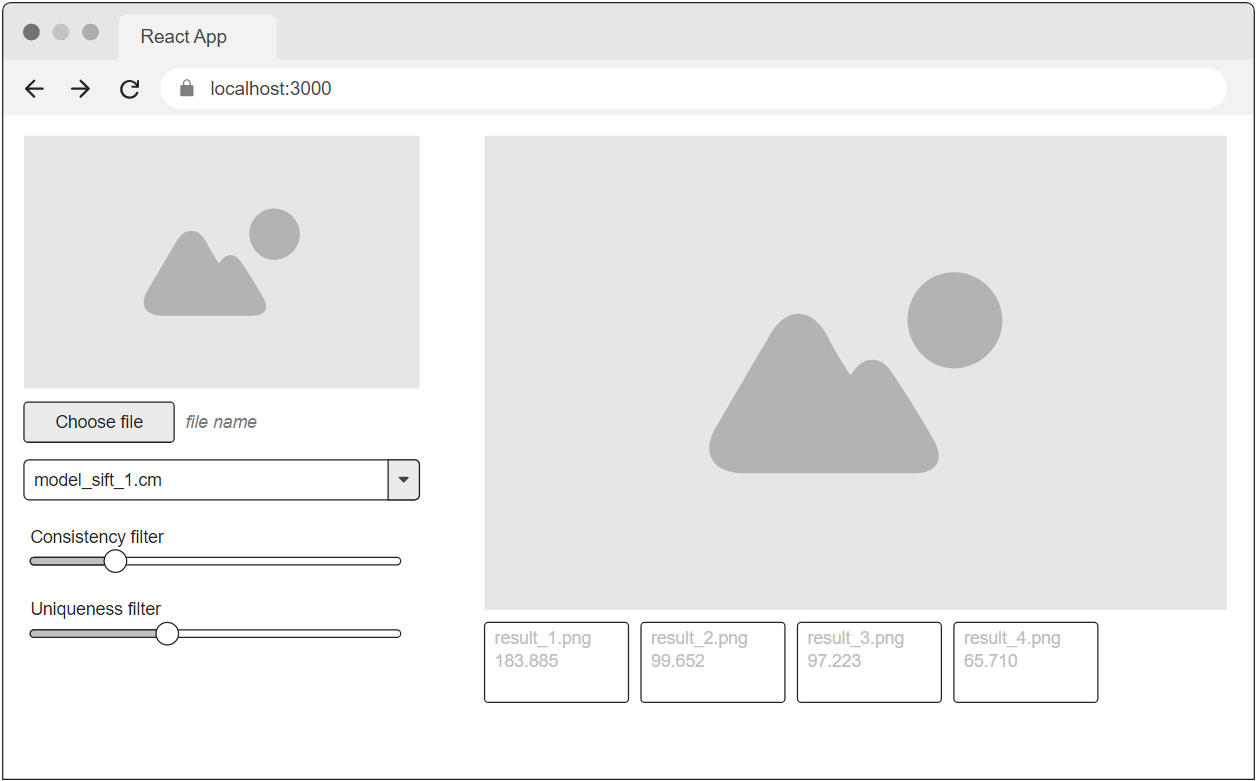
\includegraphics[width=\textwidth]{rancangan_ui.png}
	\caption{Rancangan tampilan perangkat lunak untuk BSIS.}
	\label{fig:rancangan_ui}
\end{figure}

